\documentclass[dvipsnames,svgnames]{beamer}
\usetheme{Warsaw}
\usepackage[utf8]{inputenc}
\usepackage[english]{babel}
\usepackage{amsmath}
\usepackage{amsfonts}
\usepackage{amssymb}
\usepackage{graphicx}
\usepackage[linesnumbered,ruled]{algorithm2e}
\usepackage{tikz}
\usetikzlibrary{automata, positioning}
\usepackage{float}
\usepackage[normalem]{ulem}
\usepackage{color}
\usepackage{xcolor}
\usepackage{subcaption}
\usepackage{multirow}

%Graphics and Videos
\usepackage{graphicx} %The mode "LaTeX => PDF" allows the following formats: .jpg  .png  .pdf  .mps
\graphicspath{{./video/}} %Where the figures folder is located
\usepackage{media9}
\addmediapath{./video/}

\expandafter\def\expandafter\insertshorttitle\expandafter{%
	\insertshorttitle\hfill%
    \insertframenumber\,/\,\inserttotalframenumber}



\author{Charles Dufour}
\title{Reinforcement learning and robot navigation }
%\setbeamercovered{transparent} 
\setbeamertemplate{navigation symbols}{} 
%\logo{} 
\institute{Supervisors: Prof. F. Eisenbrand, Jonas Racine} 
\date{June 20, 2018}
%\subject{} 

\newtheorem{madef}{Definition}

\begin{document}


\begin{frame}
\titlepage
\centering
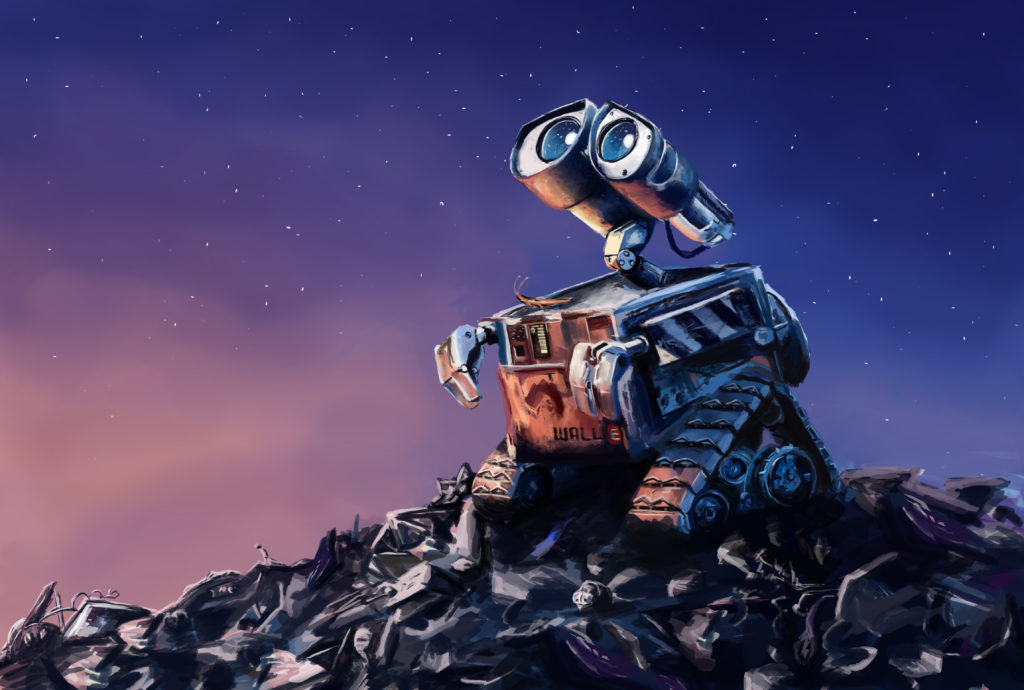
\includegraphics[scale=1]{img/Wall-E.jpg}
\end{frame}

%\begin{frame}
%\tableofcontents
%\end{frame}



\begin{frame}
\frametitle{Introduction}
\begin{block}{The problem}

  \begin{itemize}
   \item Framework: a Raspberry Pi 3 robot which can follow lines
   \item The task: the robot should adapt its speed with respect to traffic lights
   \item How: using Reinforcement Learning (RL) 
  \end{itemize}
\end{block} 
\end{frame}

\begin{frame}
\frametitle{The task}
\begin{center}
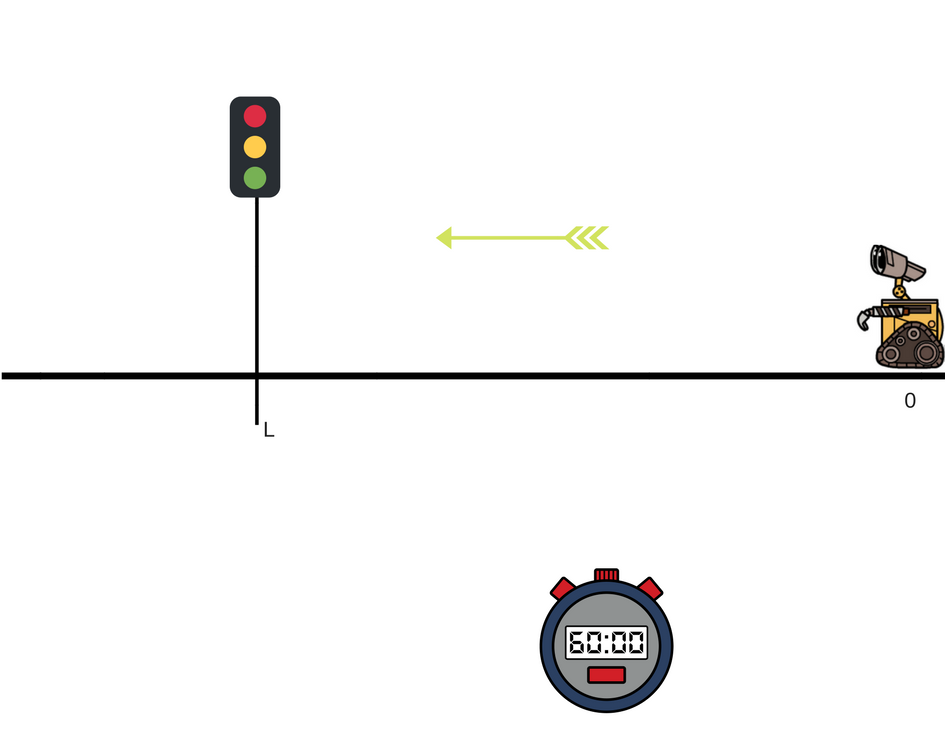
\includegraphics[scale=0.4]{img/illustration_traffic_light.png}
\end{center}
\end{frame}



\begin{frame}{Presentation}
\begin{block}{}
\begin{enumerate}
\item Reminders
\item Modeling
\item Simulation
\item Results
\end{enumerate}
\end{block}
\end{frame}

\begin{frame}
\frametitle{Reinforcement learning}
\centering
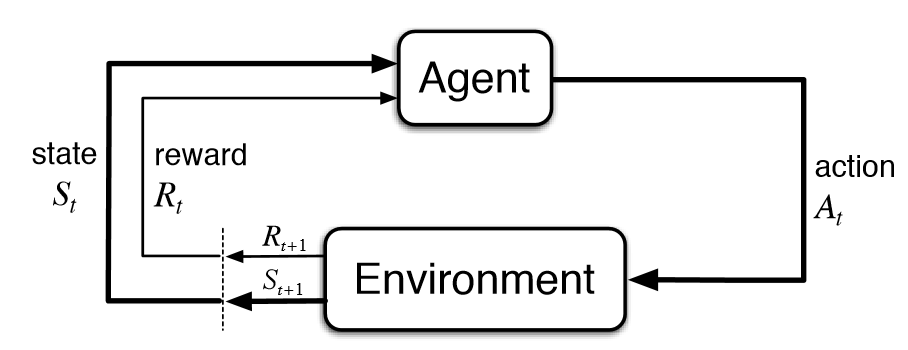
\includegraphics[scale=0.5]{img/RL_graph.png}
\vspace{1cm}

The agent's job is to find a behavior that maximizes the long-run sum of values of the rewards.
\end{frame}

\begin{frame}
\frametitle{Markov Decision Process}
\begin{block}{Definition: (MDP) }
\begin{itemize}
\item A set of states $\mathcal{S}=\{s_0,s_1,s_2,\ldots,s_{n}\}$
\item A set of actions $\mathcal{A}=\{a_1,a_2,a_3,\ldots,a_{k}\}$
\item A transition function $T(a,s,s') = \mathbb{P}[s'\mid a,s]$
\item A reward function $R: \mathcal{S} \times \mathcal{A}\mapsto \mathbb{R}$
\item A discount factor $0 \leq \gamma < 1$ 
\end{itemize}
\end{block}

\begin{block}{Q-learning}
Approximation $Q(s,a)$ (measure "how good is the action")

Action chosen: $\underset{a}{\text{argmax }}Q(s,a)$
\end{block}
\end{frame}

\begin{frame}
\frametitle{Modeling}
\begin{block}{States}
States encode the following information:
\begin{itemize}
\item distance to the traffic light
\item speed 
\item color of the traffic light
\item time spent in current color 
\item previous action 
\end{itemize}
\end{block}
\end{frame}



\begin{frame}
\frametitle{Modeling}
\begin{block}{Actions}
\begin{itemize}
\item slow down
\item keep the same speed 
\item speed up
\end{itemize}
\end{block}
Possible speeds: $0, 20, 30, \ldots, 70$
\end{frame}
%
%\begin{frame}
%\frametitle{Modeling}
%\framesubtitle{Actions effect: acceleration}
%\begin{tikzpicture}[font=\sffamily]
%    % Add the states
%        %\node[state,draw=none] (d1) [left of=1] {};
%        \node[state,text = black
%              ] (h0) {$d_0$};
%		\node[state,
%			below=1 cm of h0,
%			text = black
%        	] (m0) {$d_0$};
%		\node[state,
%			below= 1 cm of m0,
%        	text=black,
%        	] (l0) {$d_0$};
%         \node[state,
%         	 right = 1 cm of h0,
%             text = black
%              ] (h1) {$d_1$};	
%		\node[state,
%			below=1 cm of h1,
%        	text = black
%        	] (m1) {$d_1$};
%		\node[state,
%			below= 1 cm of m1,
%        	text=black,
%        	] (l1) {$d_1$};
%         \node[state,
%         	right = 1 cm of h1,
%         	text = black
%              ] (h2) {$d_2$};	
%		\node[state,
%			below=1 cm of h2,
%        	text = black,
%        	] (m2) {$d_2$};
%		\node[state,
%		below= 1 cm of m2,
%        	text=black,
%        	] (l2) {$d_2$};
%        \node[state,
%        	right = 1 cm of h2,
%        	text = black
%             ] (h3) {$d_3$};	
%		\node[state,
%			below=1 cm of h3,
%        	text=black
%        	] (m3) {$d_3$};
%		\node[state,
%			below= 1 cm of m3,
%        	text=black,
%        	] (l3) {$d_3$};   	
%		\node[state,draw=none] (d1) [right = 1 cm of l3] {};	
%		\node[state,draw=none] (d2) [right = 1 cm of m3] {};
%		\node[state,draw=none] (d3) [right = 1 cm of h3] {};
%		\node[state,draw=none] (d4) [right = 1 cm of d3] {};
%		\node[draw=none] (legend1) [left=0.3 cm of l0] {speed n};
%		\node[draw=none] (legend2) [left = 0.3 cm of m0] {\textcolor{black}{speed n+10}};
%		\node[draw=none] (legend3) [left = 0.3 cm of h0] {\textcolor{black}{speed n+20}};
%		        
%       \draw[every loop,
%        auto=right,
%        >=latex,
%        draw=black!60,
%        fill=black!60]
%			(l0) edge[](l1)
%			(l1) edge[] (l2)	
%			(l2) edge[] (l3)
%			(l3) edge[dashed] (d1)
%			(m0) edge[bend left] (m2)
%			(m1) edge[bend left] (m3)
%			(m2) edge[bend left,dashed] (d2)
%			(h0) edge[bend left] (h3)
%			(h1) edge[bend left,dashed] (d3)
%            ;
%      \draw[every loop,
%        auto=right,
%        >=latex,
%        draw=red,
%        fill=red]
%			(l0) edge[](m2)
%			(l1) edge[] (m3)	
%			(m0) edge[] (h3)
%			(h0) edge[bend left] (h3)
%			(h1) edge[bend left,dashed] (d3)
%			(l2) edge[dashed] (d2)
%			(m1) edge[dashed] (d3);
%	\end{tikzpicture}
%\end{frame}

\begin{frame}
\frametitle{Modeling}
\framesubtitle{classical reward function, naive thinking}
\begin{block}{Reward function: $\mathcal{R}(s,a)$}
\begin{itemize}
\item positive reward if robot respects the traffic light
\item negative reward for every step "far away" from the traffic light
\end{itemize}
\end{block}

Positive reward when the task is done and negative reward for every step along the way.
\end{frame}


\begin{frame}
\frametitle{Simulation}
\framesubtitle{Questions}
\begin{block}{}
\begin{itemize}
\item how to compute the distance from the robot to the traffic light? 
\item how "fast" is speed $20, 30, \ldots$? 
\item how to simulate the traffic light? 
\item what are the exact parameters for the reward function? 
\end{itemize}
\end{block}
\vspace{1cm}
\end{frame}

\begin{frame}
\frametitle{Simulation}
\framesubtitle{Measuring distance to the traffic light}
\begin{figure}[H]
\captionsetup{justification=centering,margin=0cm}
\centering
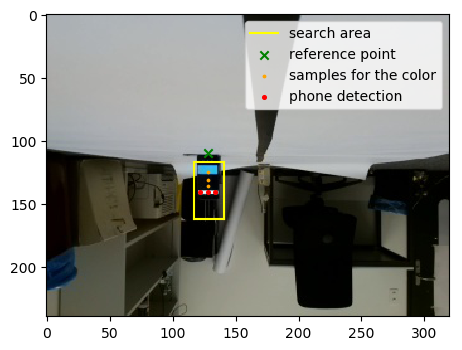
\includegraphics[scale=0.7]{img/vue46.png}
\caption{View from the robot camera}
\end{figure}
\end{frame}

\begin{frame}
\frametitle{Simulation}
\framesubtitle{Measuring distance to the traffic light}
\begin{figure}[H]
\captionsetup{justification=centering,margin=0cm}
\centering
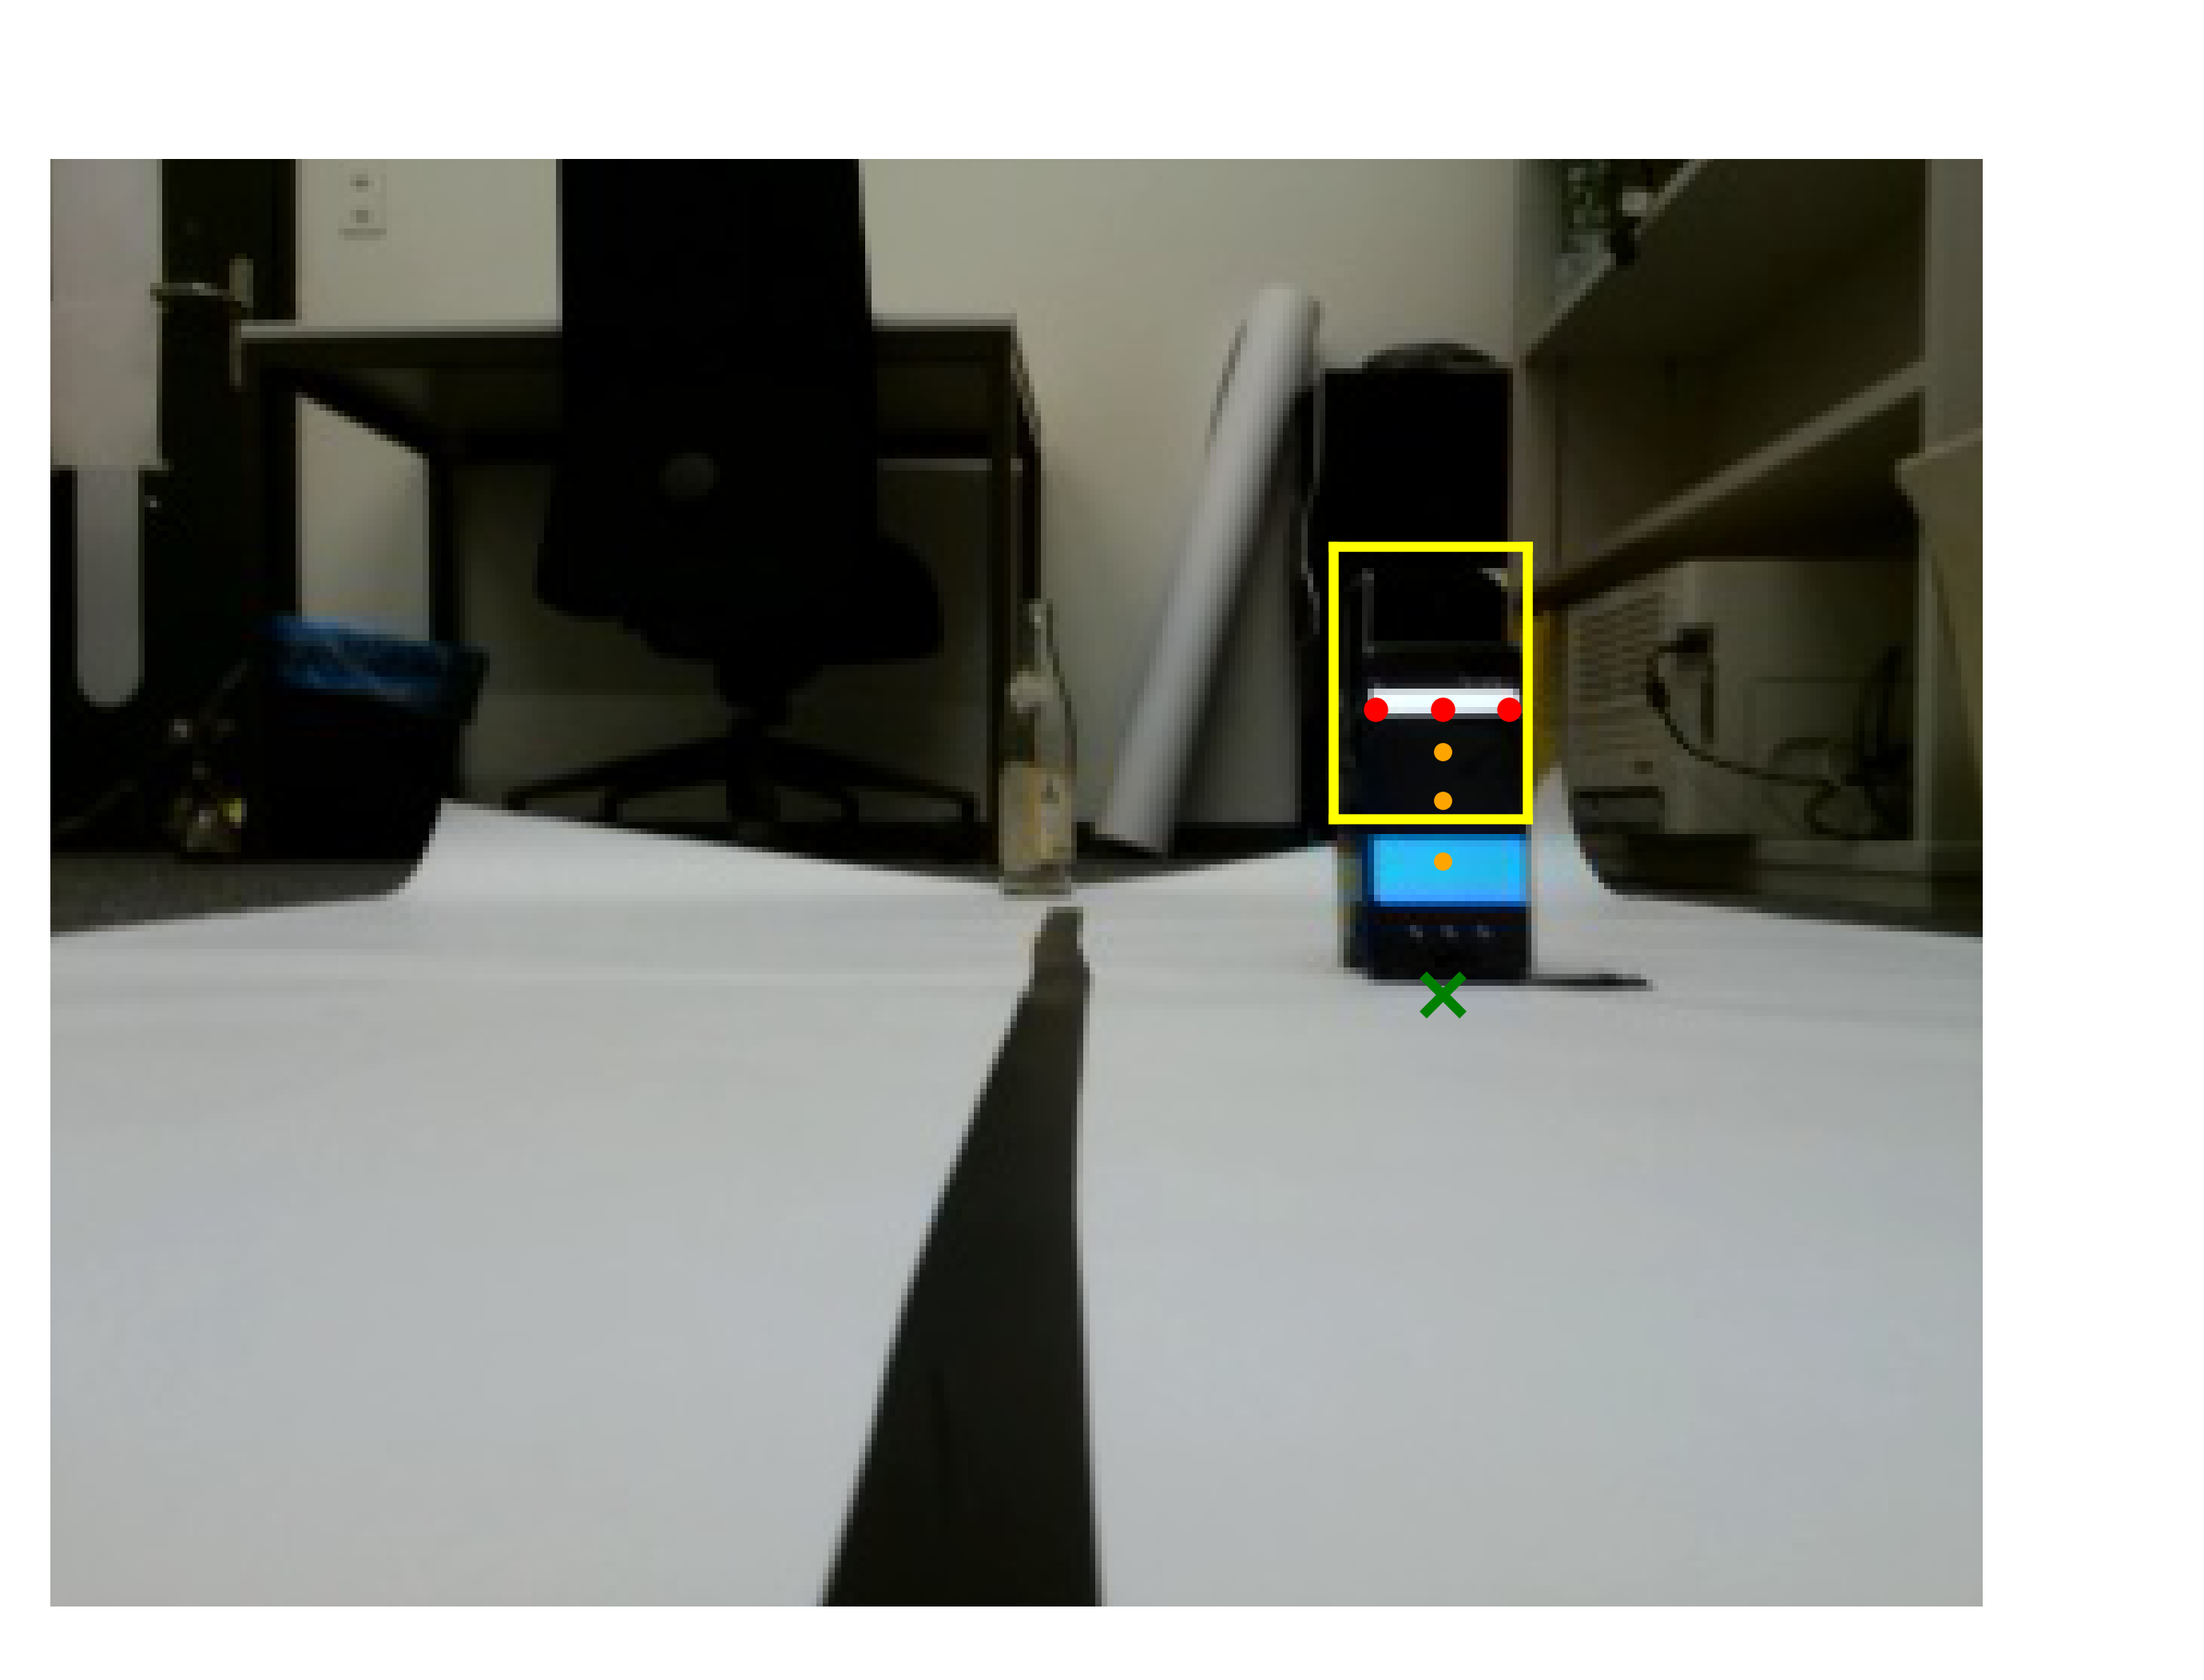
\includegraphics[scale=0.7]{img/rotated-img38.png}
\caption{View from the robot camera}
\end{figure}
\end{frame}



\begin{frame}
\frametitle{Simulation}
\framesubtitle{measuring distance from the robot to the traffic light}
\center
\begin{figure}[ht]
        \centering
        \captionsetup{justification=centering,margin=2cm}

        \begin{subfigure}[b]{0.4\textwidth}
            \centering
            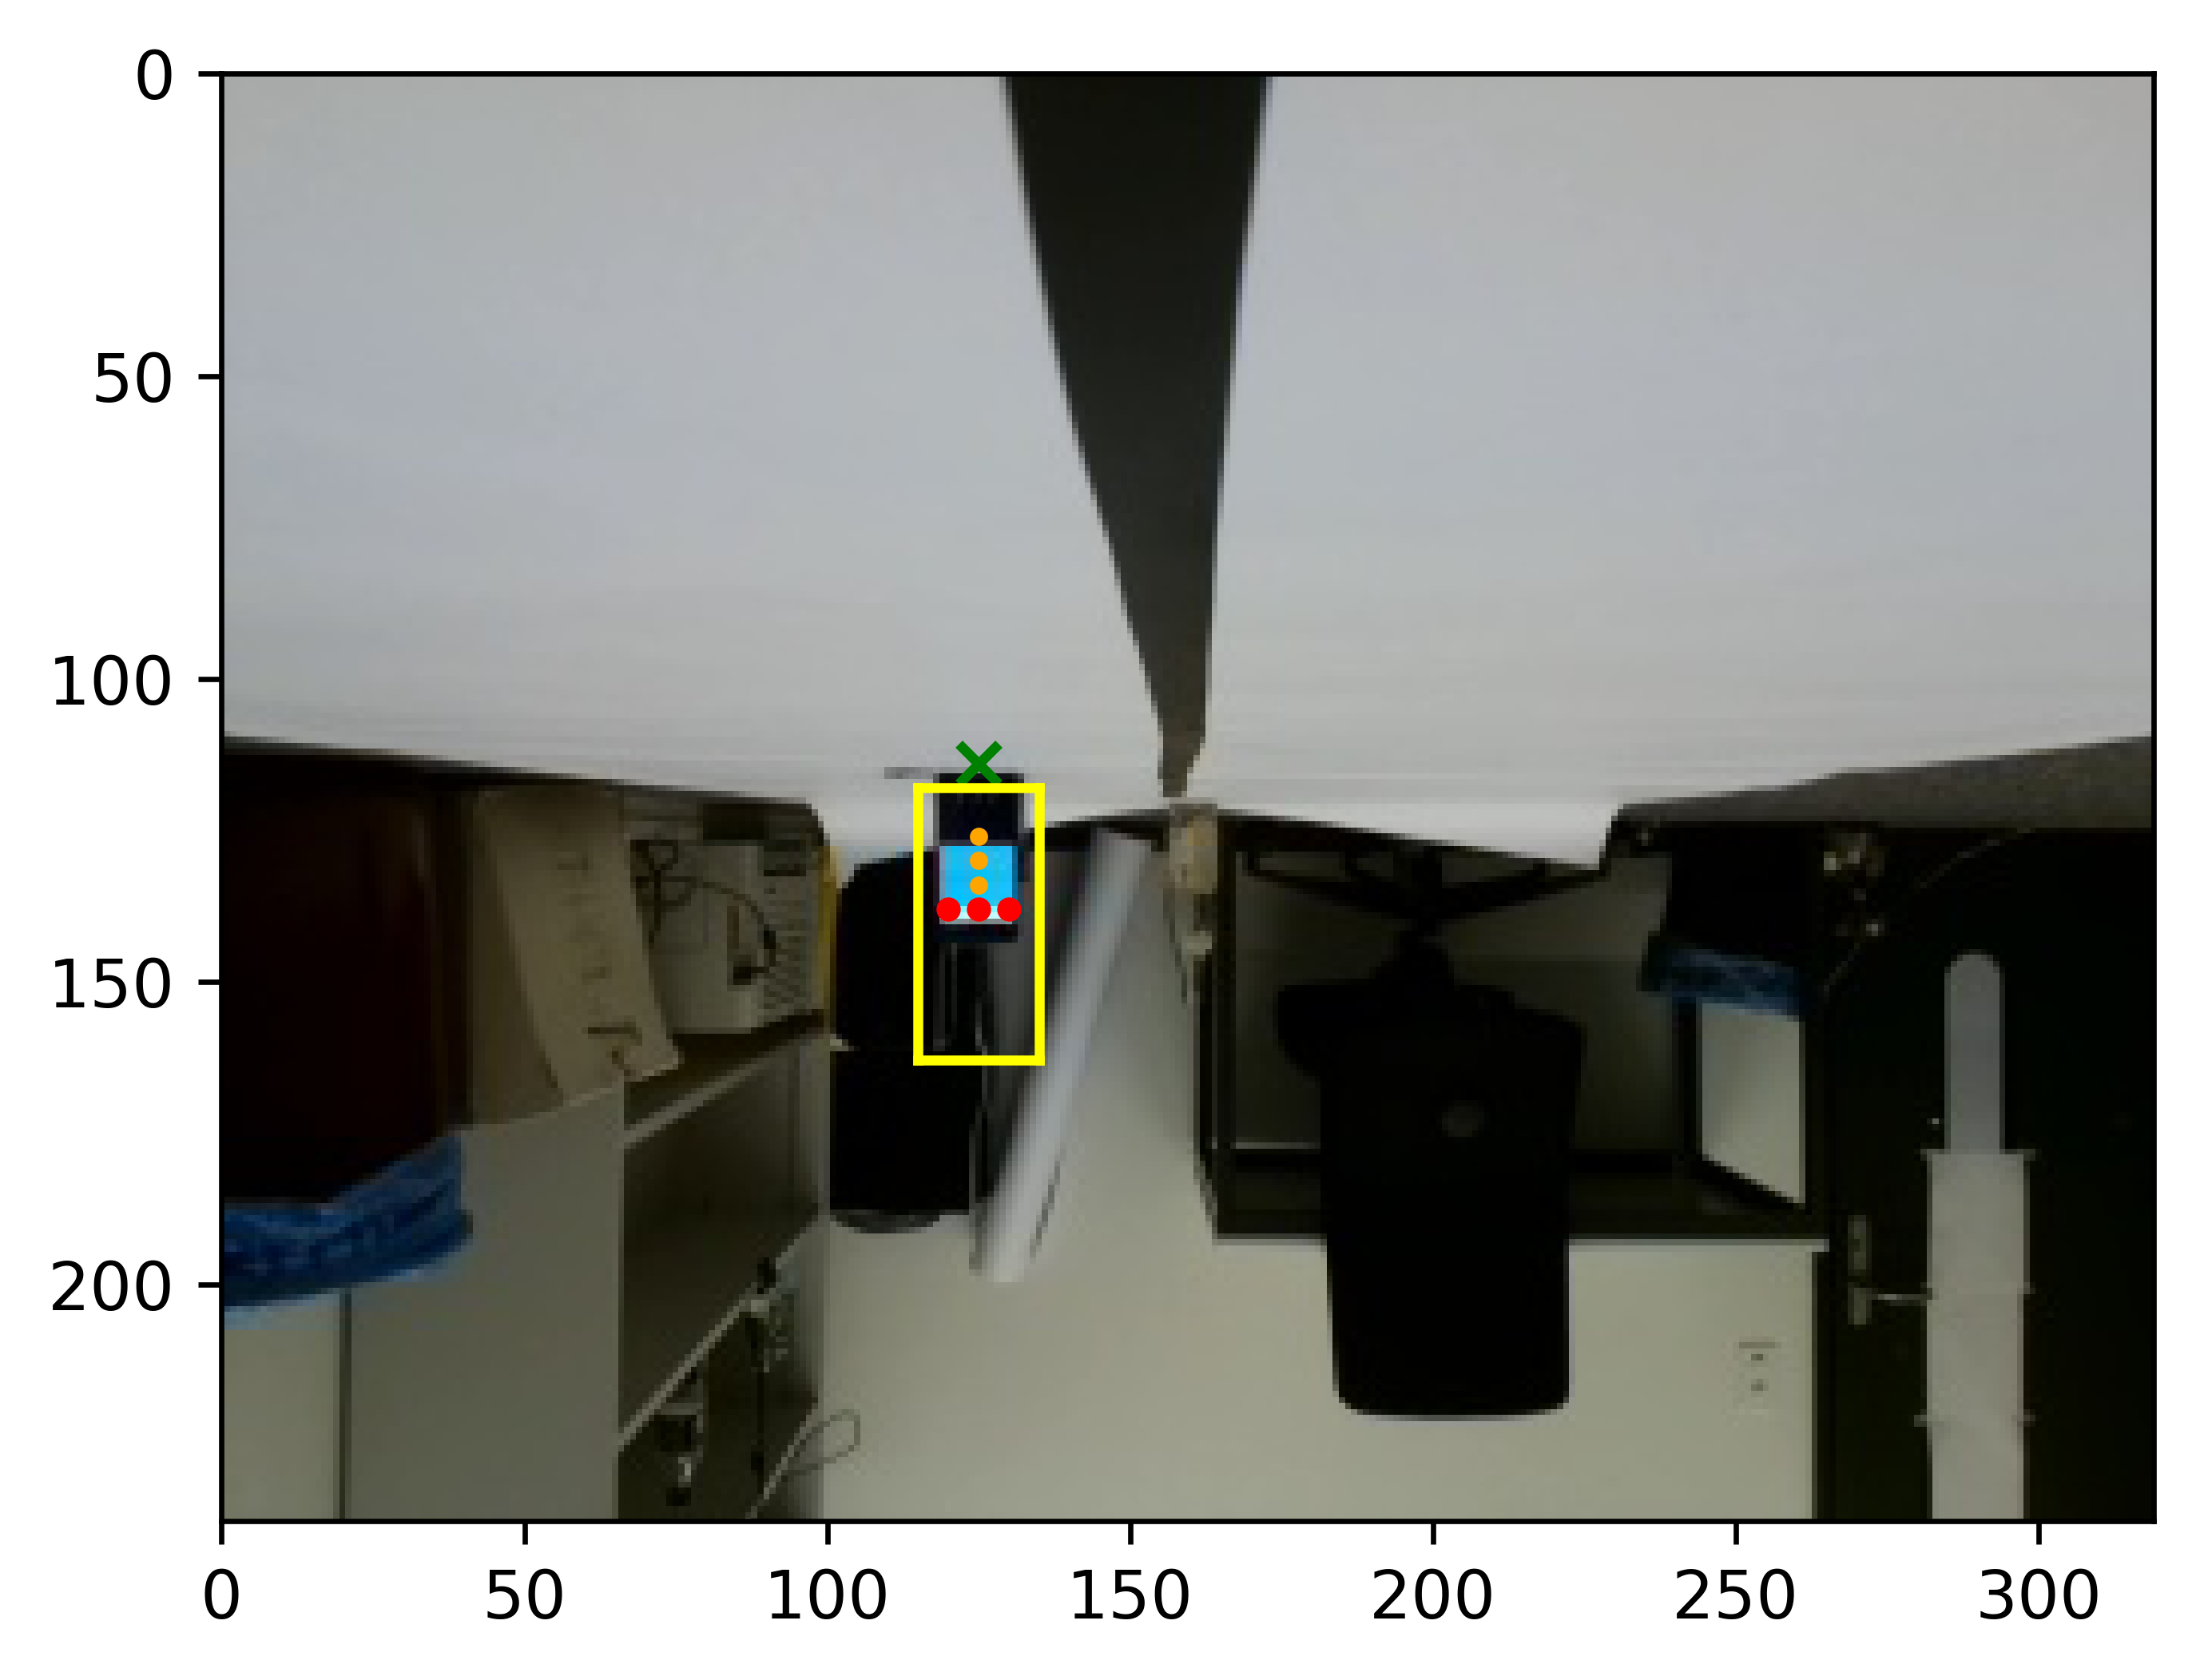
\includegraphics[width=\textwidth]{video/img07.png}   
            \label{fig:mean and std of net14}
        \end{subfigure}
        \begin{subfigure}[b]{0.4\textwidth}  
            \centering 
            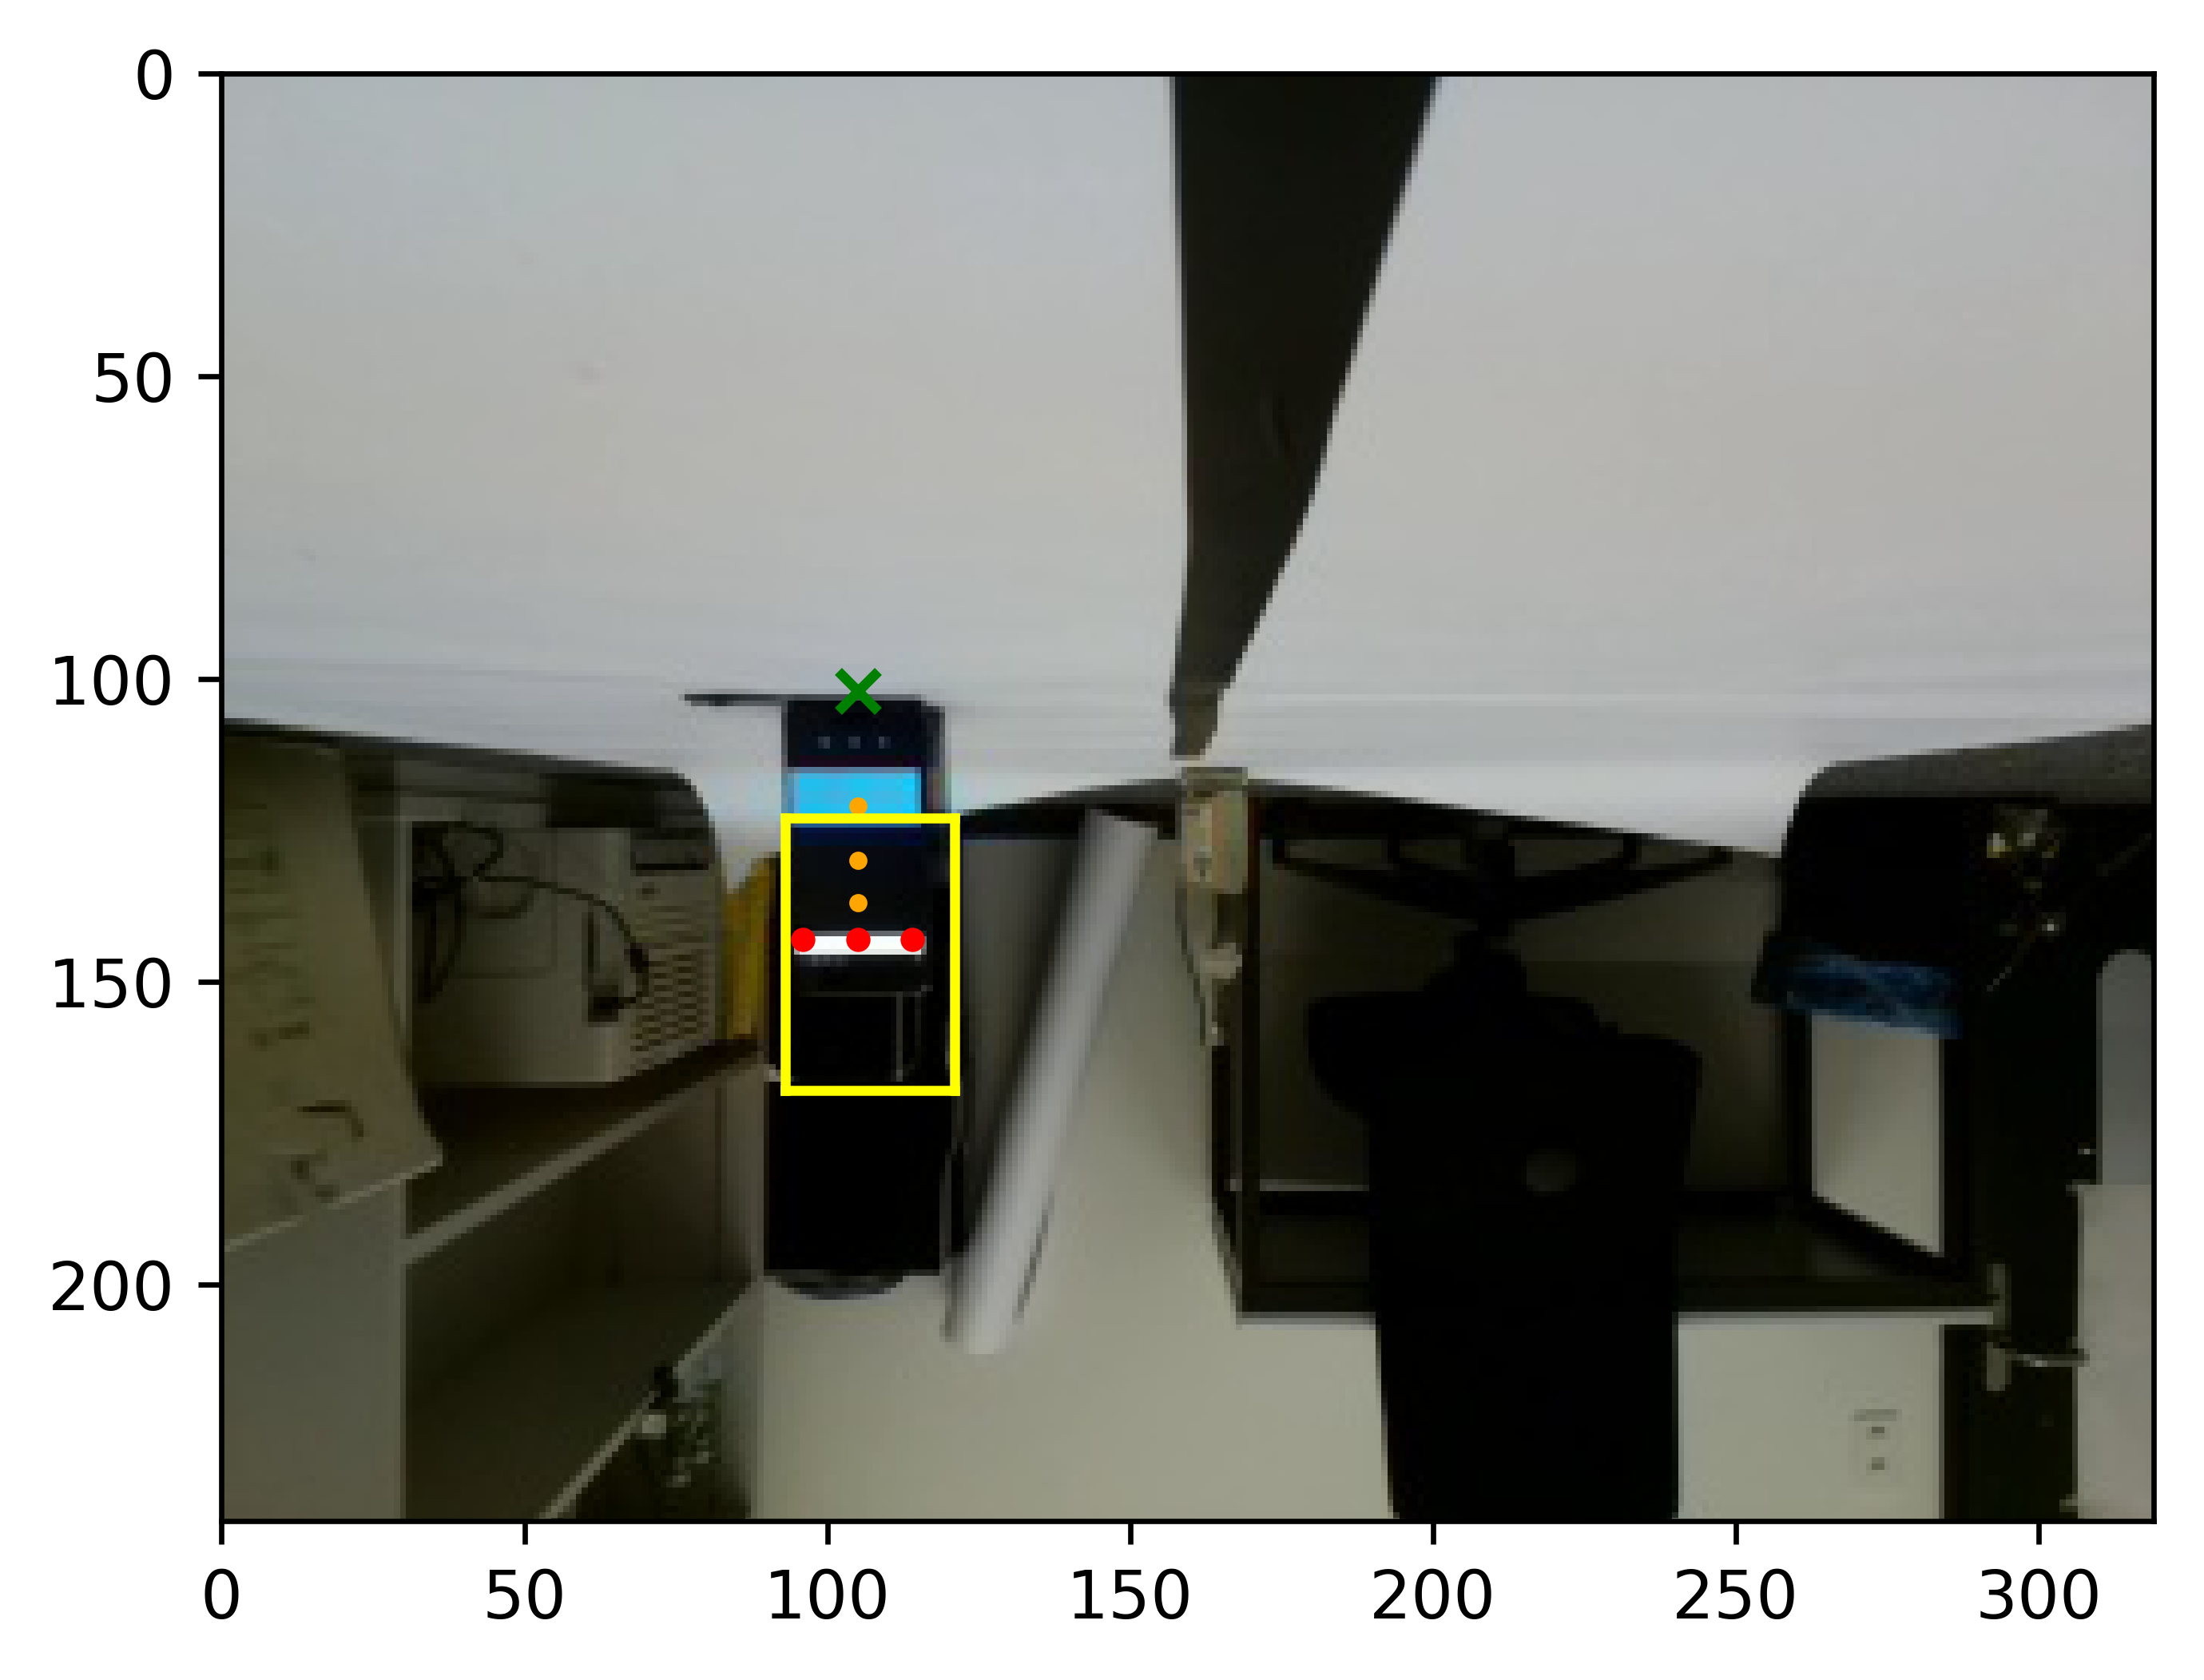
\includegraphics[width=\textwidth]{video/img30.png}
            \label{fig:mean and std of net24}
        \end{subfigure}
        \vskip\baselineskip
        
        \begin{subfigure}[b]{0.4\textwidth}   
            \centering 
            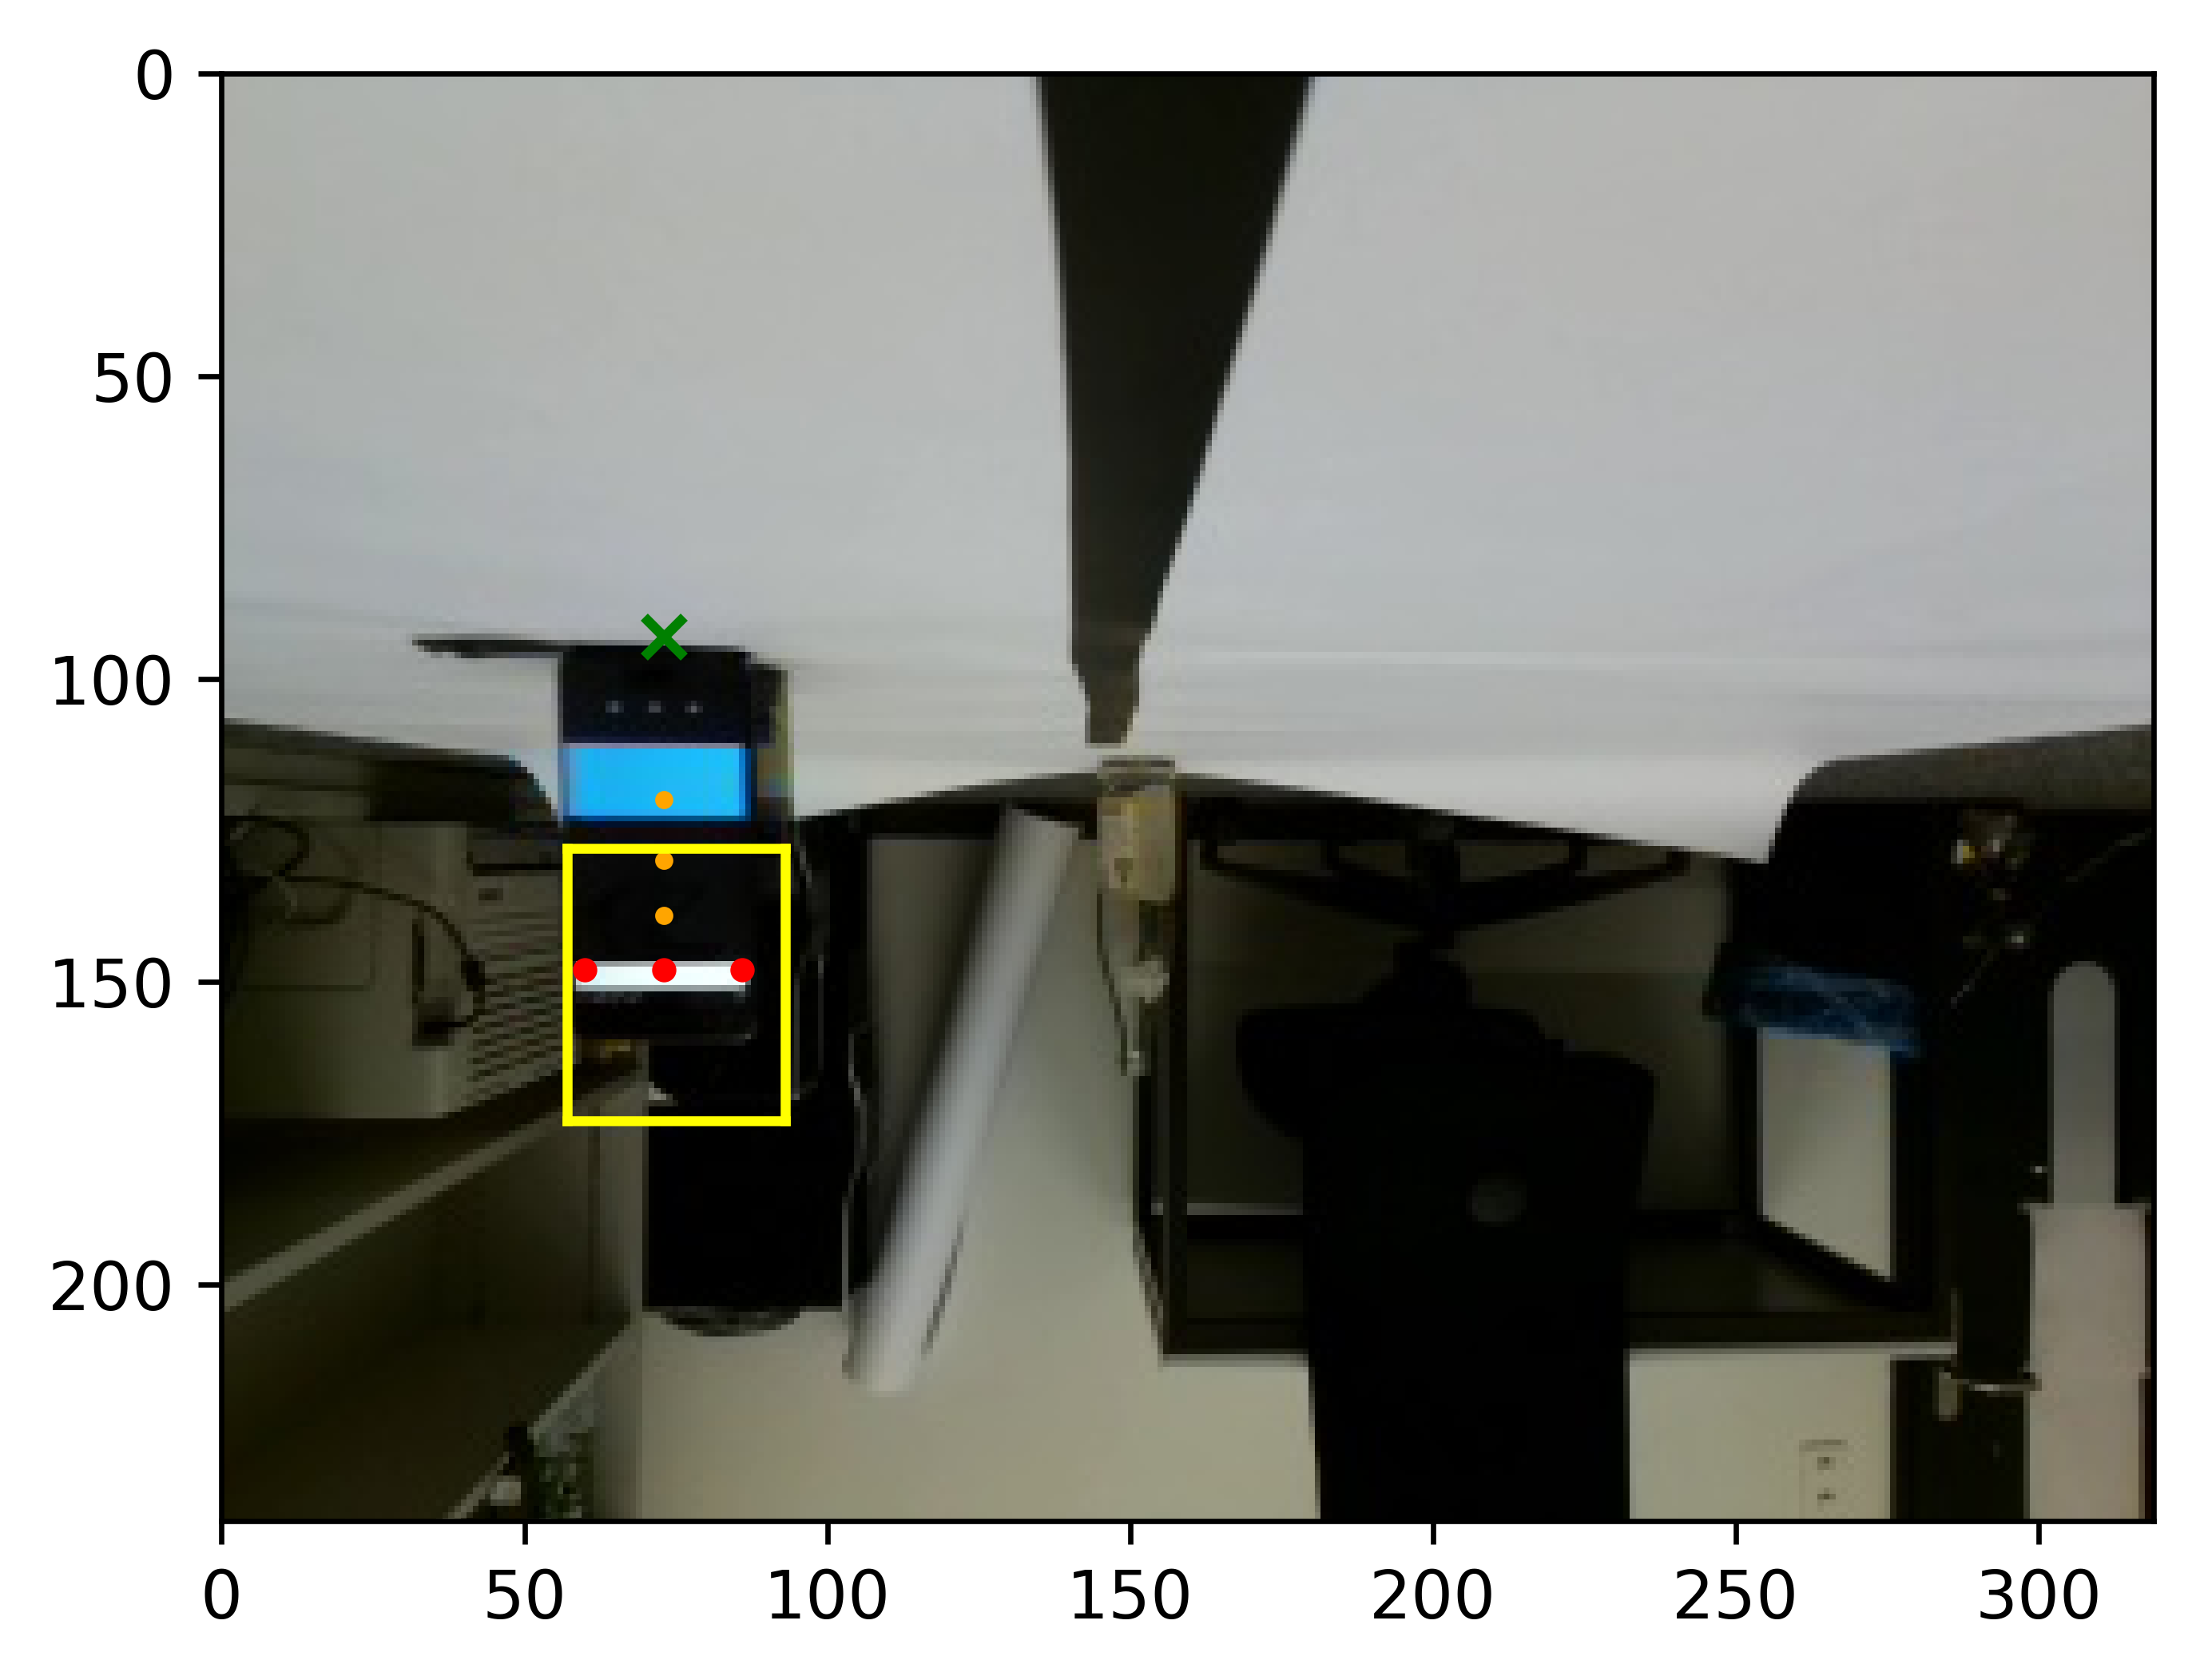
\includegraphics[width=\textwidth]{video/img46.png}
   
            \label{fig:mean and std of net34}
        \end{subfigure}
        \begin{subfigure}[b]{0.4\textwidth}   
            \centering 
            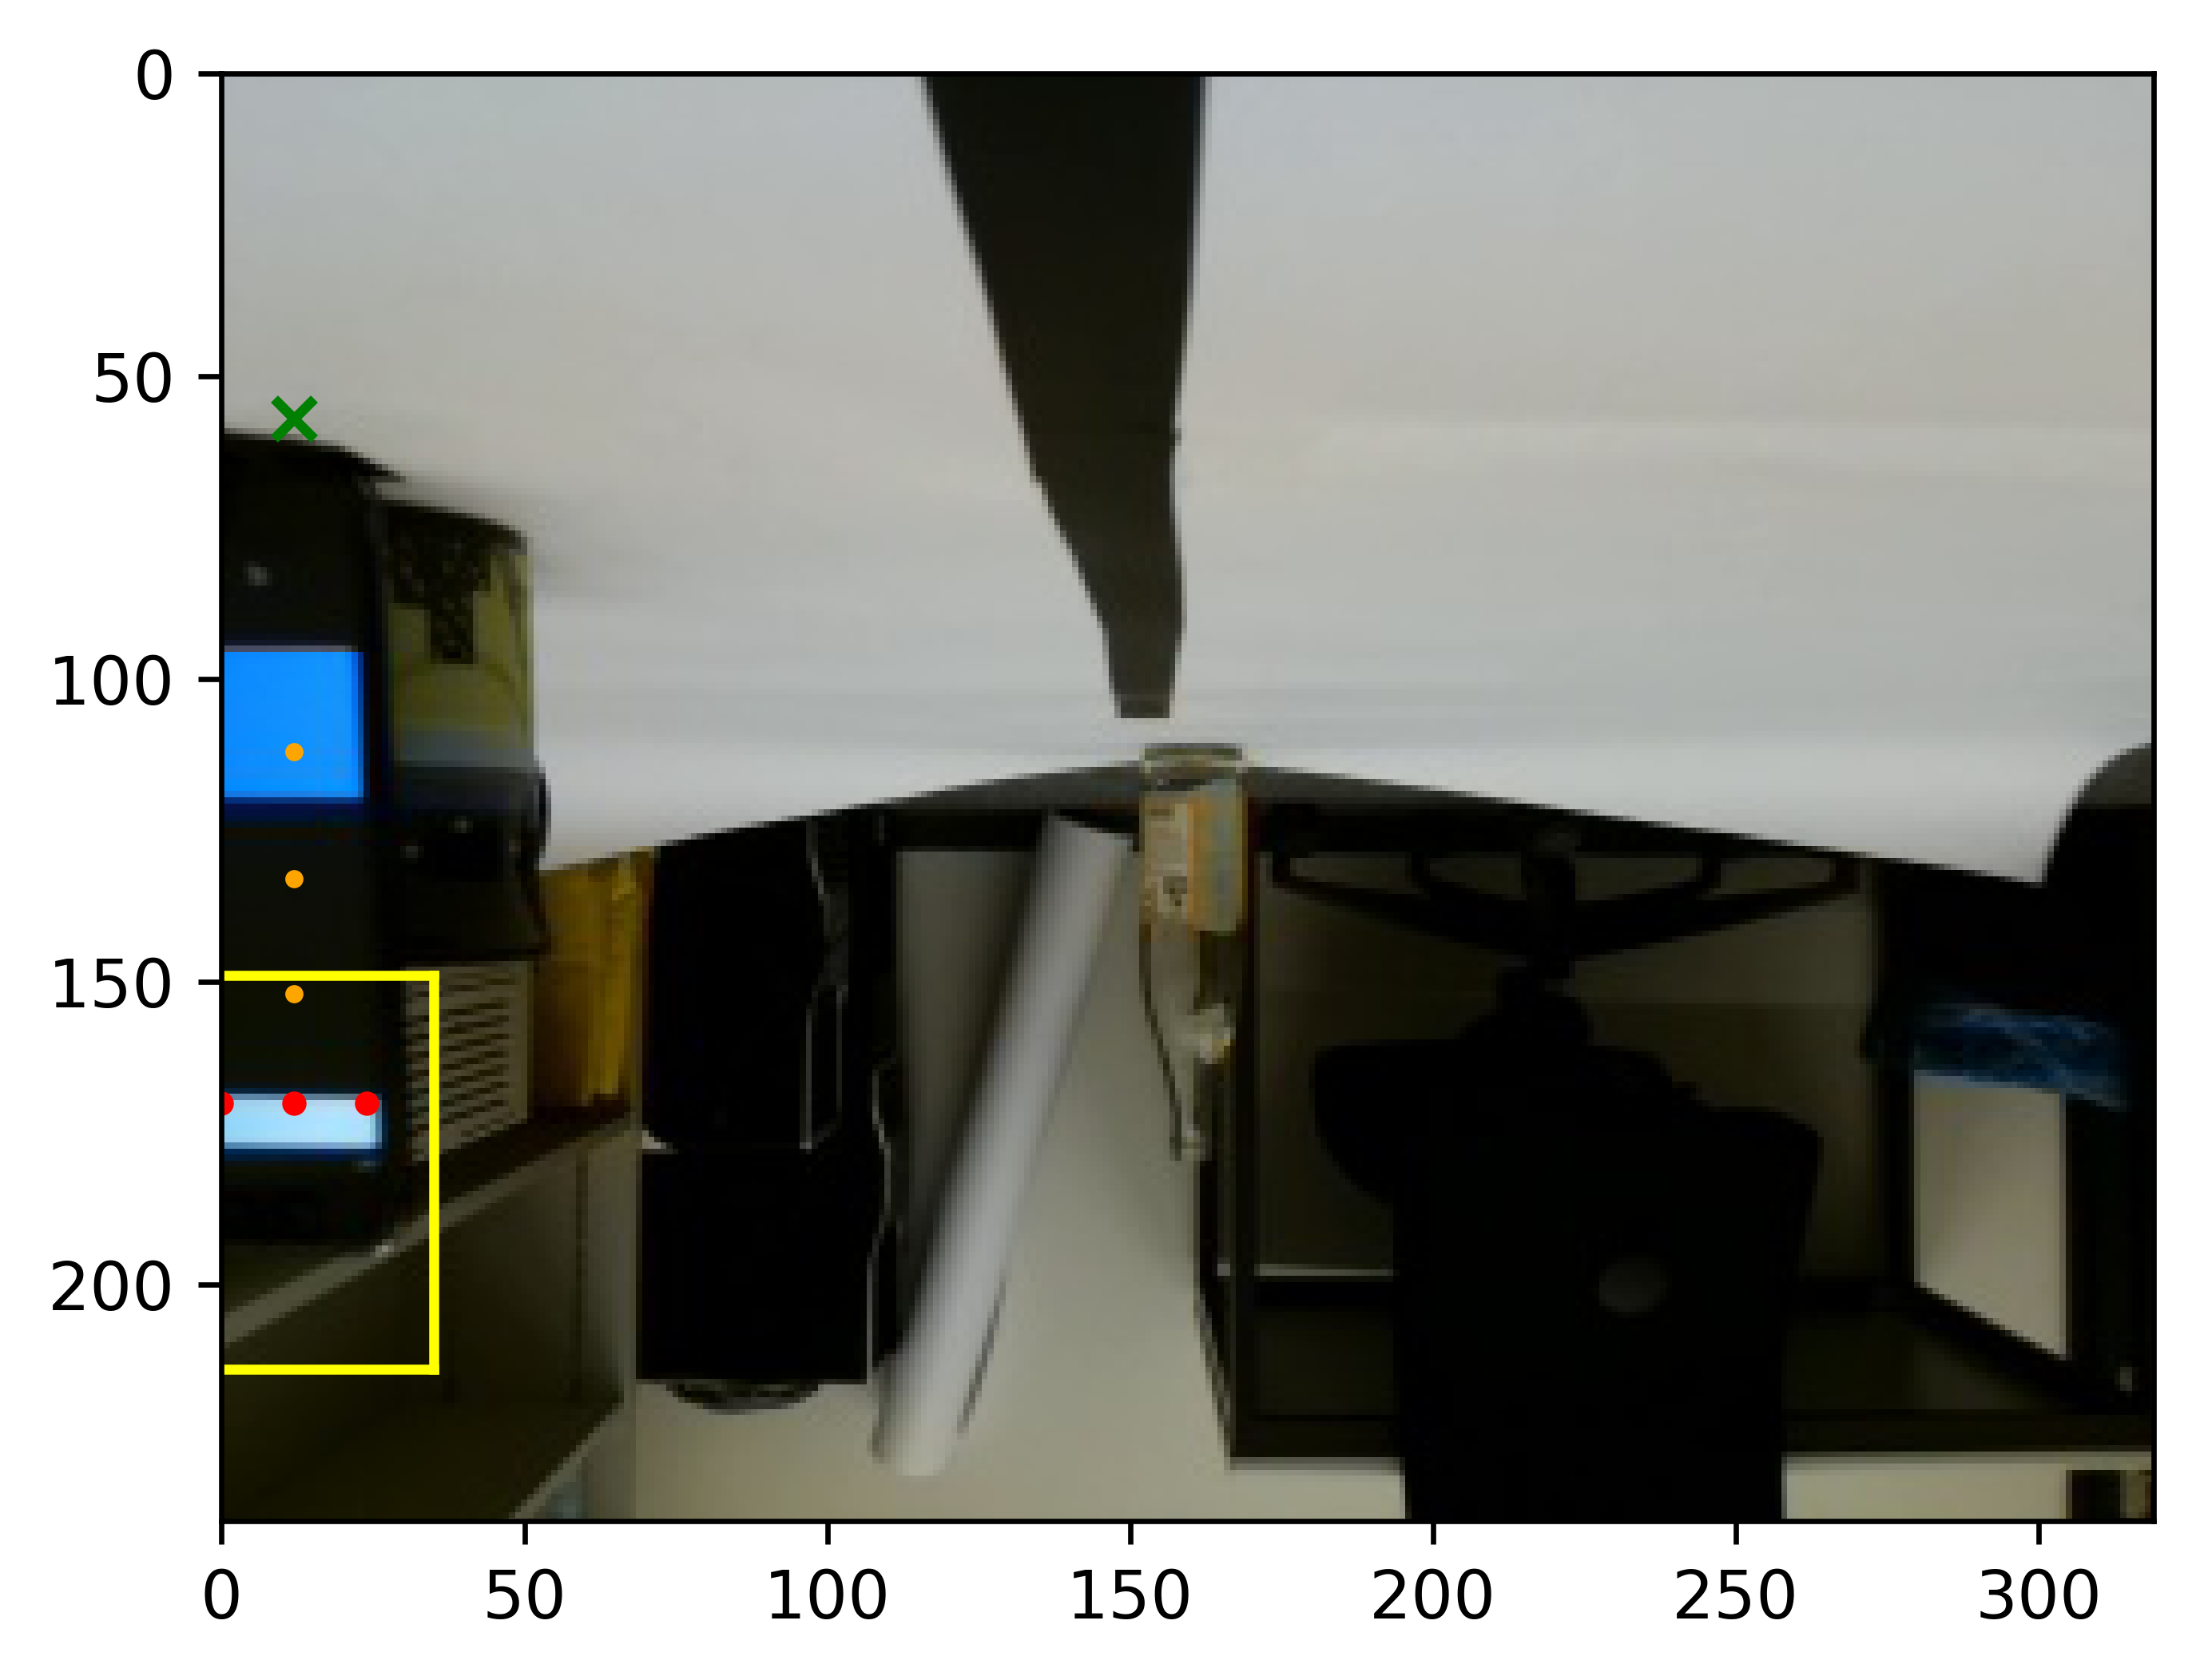
\includegraphics[width=\textwidth]{video/img60.png}
  
            \label{fig:mean and std of net44}
        \end{subfigure}
\end{figure}
\end{frame}

\begin{frame}
\frametitle{Simulation}
\framesubtitle{How fast is fast? Graphs for speed 30 and 70 }

\begin{figure}[ht]
        \centering
        \captionsetup{justification=centering,margin=2cm}
        \begin{subfigure}[b]{0.7\textwidth}
            \centering
            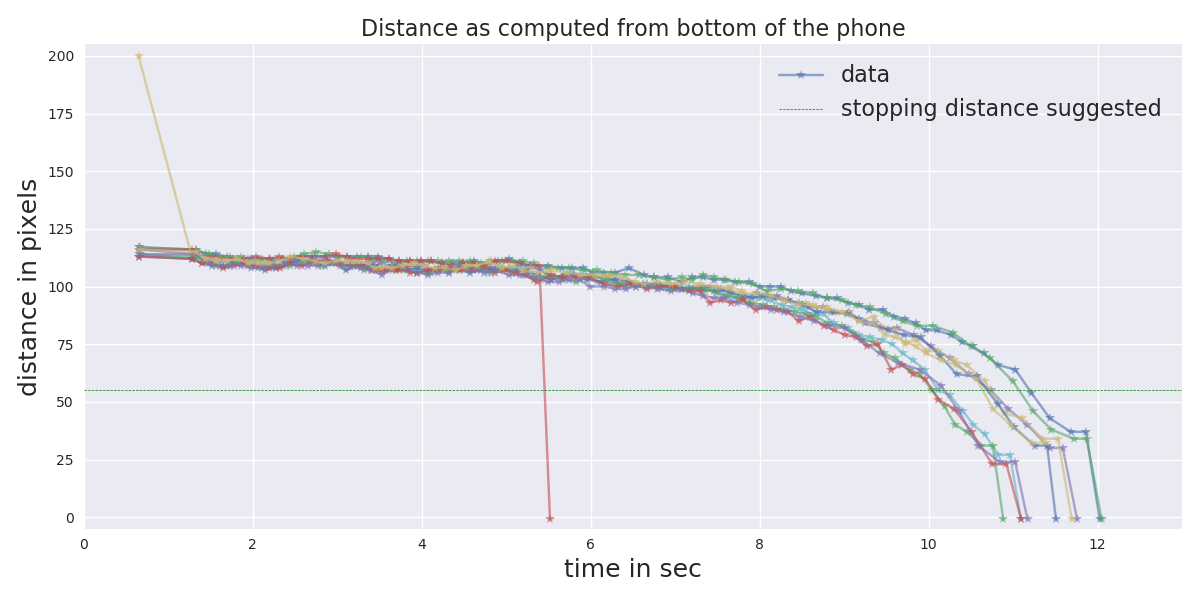
\includegraphics[width=\textwidth]{img/distances_30.png}   
        \end{subfigure}
        
        
        \begin{subfigure}[b]{0.7\textwidth}  
            \centering 
            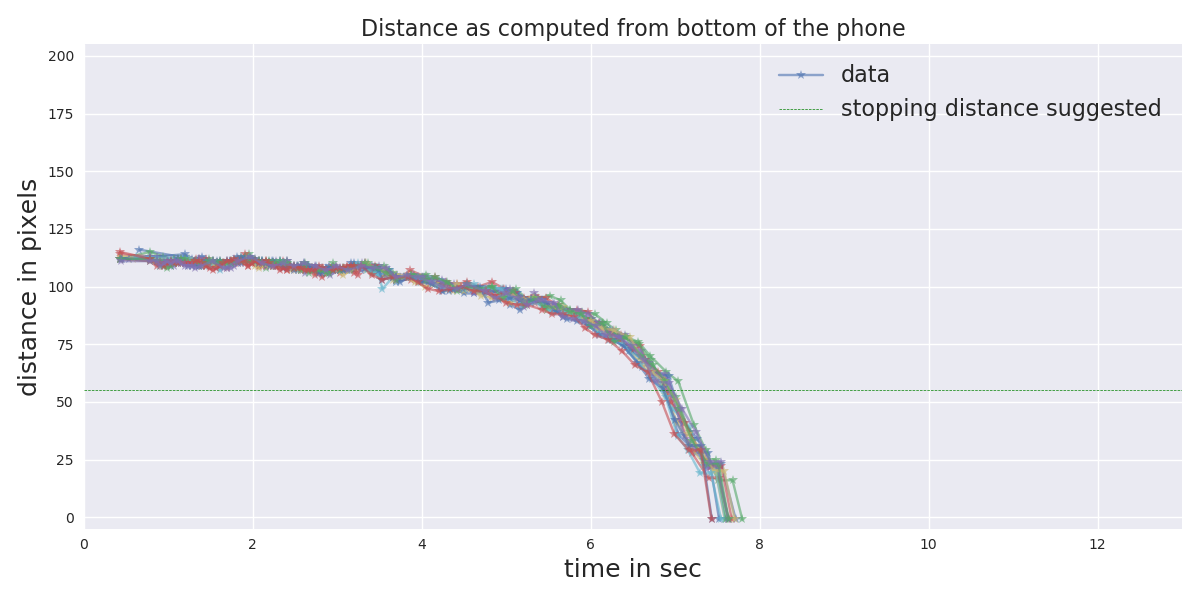
\includegraphics[width=\textwidth]{img/distances_70.png}
        \end{subfigure}
\end{figure}

\end{frame}


\begin{frame}{Simulation}{Imputation of missing data for a fixed speed $v$}

\begin{table}[]
\centering
\caption{Example of raw data obtained}
\label{my-label}
\begin{tabular}{|l|l|l|l|}
\hline
position & \multicolumn{3}{l|}{outcomes} \\ \hline
80       & 75       & 74       & 73      \\ \hline
81       &          &          &         \\ \hline
82       & 76       & 77       &         \\ \hline
\end{tabular}
\end{table}

\pause 
Mean of data from the surrounding points: 75
\pause
\begin{table}[]
\centering
\caption{After imputation}
\label{my-label}
\begin{tabular}{|l|l|l|l|}
\hline
position & \multicolumn{3}{l|}{outcomes} \\ \hline
80       & 75       & 74       & 73      \\ \hline
81       & 75       & 74       &76        \\ \hline
82       & 76       & 77       &         \\ \hline
\end{tabular}
\end{table}
\end{frame}


\begin{frame}{Simulation}{Finding probabilities from the data for a fixed speed $v$}

\begin{table}[]
\centering
\caption{Example of data}
\begin{tabular}{|l|l|l|l|l|l|}
\hline
position & \multicolumn{5}{c|}{outcomes} \\ \hline
80       & 75   & 74  & 74  & 73  & 75  \\ \hline
\end{tabular}
\end{table}
\pause

\begin{table}[]
\centering
\caption{Probabilities of transitions obtained from the data}
\label{my-label}
\begin{tabular}{|c|c|c|}
\hline
from & to & probabilities \\ \hline
\multirow{3}{*}{80} & 75 & 0.4 = 2/5 \\ \cline{2-3} 
 & 74 & 0.4 = 2/5 \\ \cline{2-3} 
 & 73 &  0.2 = 1/5  \\ \hline
\end{tabular}
\end{table}

\end{frame}






\begin{frame}
\frametitle{Simulation}
\framesubtitle{Traffic light}
In the simulation, the time is defined in terms of number of interactions.
\pause

We simulated the traffic light in the following way:
\begin{itemize}
\item We measured the number of pictures processed per second by the robot ($\sim 8 $ im/s)
\item \pause Learning for a specific traffic light 
\item \pause Traffic light simulated to behave the same as in real life in terms of \emph{time} 
\end{itemize}
\end{frame}



\begin{frame}
\frametitle{Simulation}
\framesubtitle{Reward function}

\begin{block}{Issues with previous naive thinking}
\begin{itemize}
\item The distance measurements are approximative, hence we cannot have a fixed distance to stop, so we use a \emph{stopping zone}.
\item Reward functions are not as simple as they seem. We had to test a lot of them, small changes have influence \ldots
\end{itemize}
\end{block}
\end{frame}

\begin{frame}
\frametitle{Simulation}
\framesubtitle{Reward function, naive approach 1 million episodes}

\centering
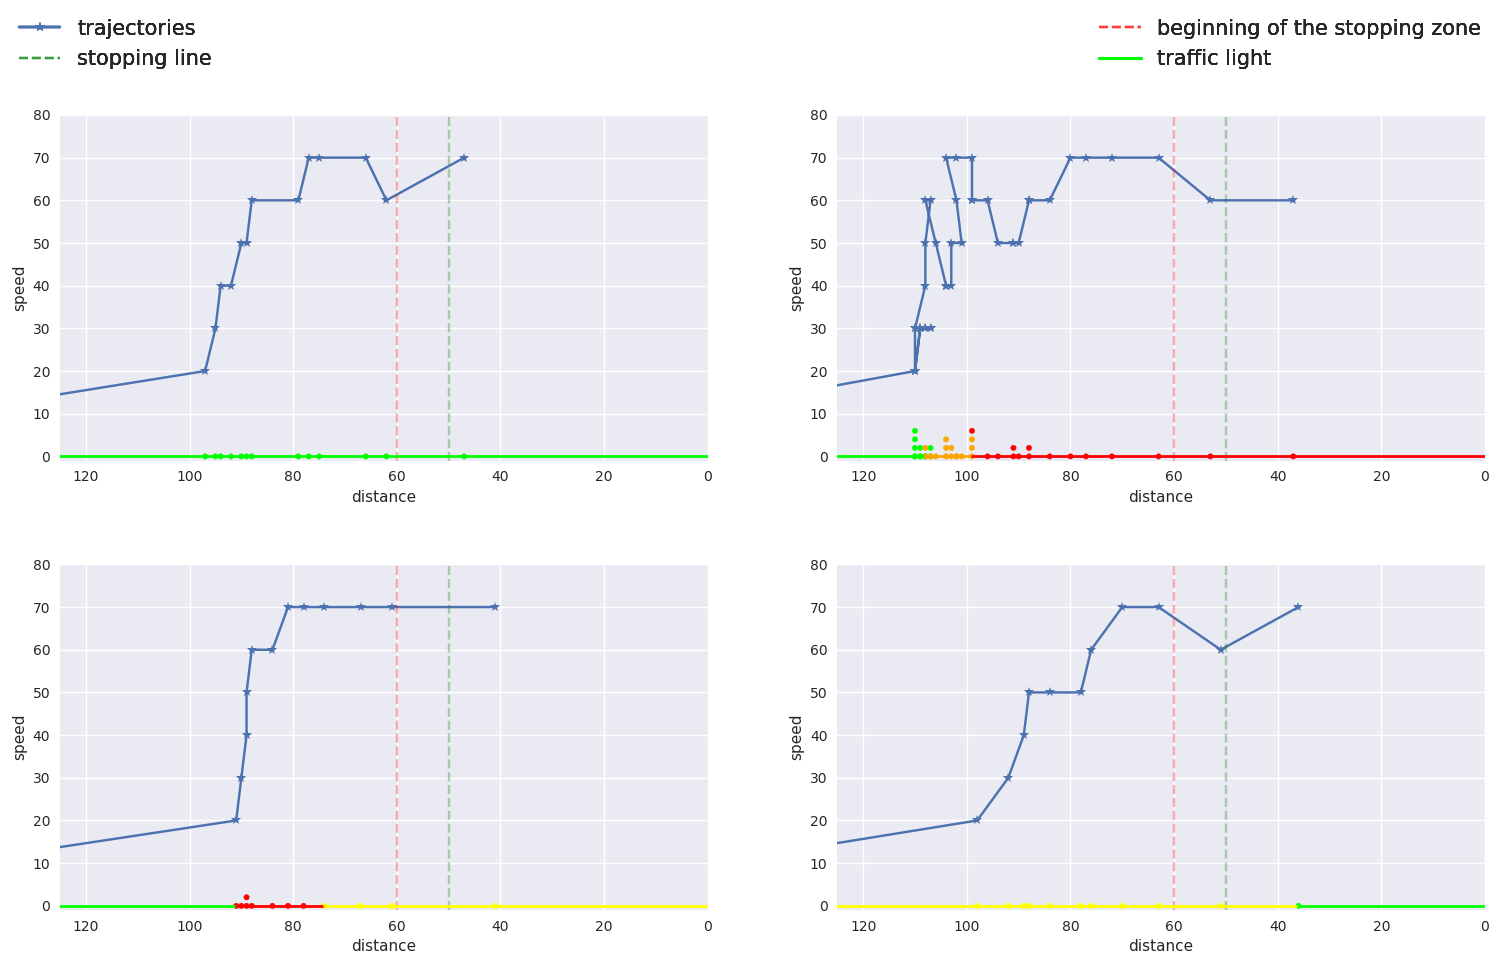
\includegraphics[scale=0.3]{img/new_legend_traj_weak.png}

\end{frame}

\begin{frame}
\frametitle{Simulation}
\framesubtitle{Reward function}
\begin{block}{Solutions}
\begin{itemize}
\item  add great negative or positive reward for respecting or not red light ($\sim \pm 300$)
\item \pause try to bait the robot to learn what we want
\item \pause and try a lot of times different reward functions (maybe 20) with a lot of iterations ($\sim 10$ millions, about half a day)
\end{itemize}
\end{block}
\end{frame}


\begin{frame}
\frametitle{Results}
 \framesubtitle{Learning curve}
 \begin{figure}
 \centering
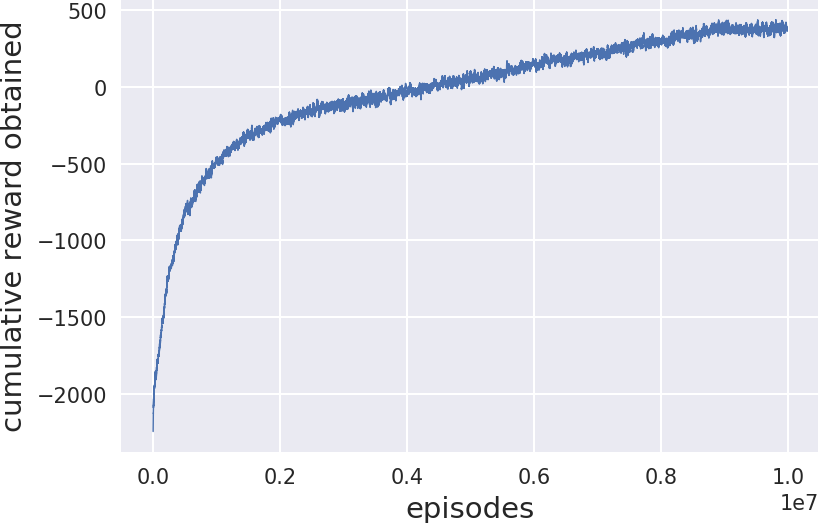
\includegraphics[scale=0.5]{img/Q-learning-curve.png}
\caption{Q-learning curve (10 millions iterations)}
\end{figure}
\end{frame}

\begin{frame}
\frametitle{Results}
 \framesubtitle{Examples of trajectories obtained}
  \centering
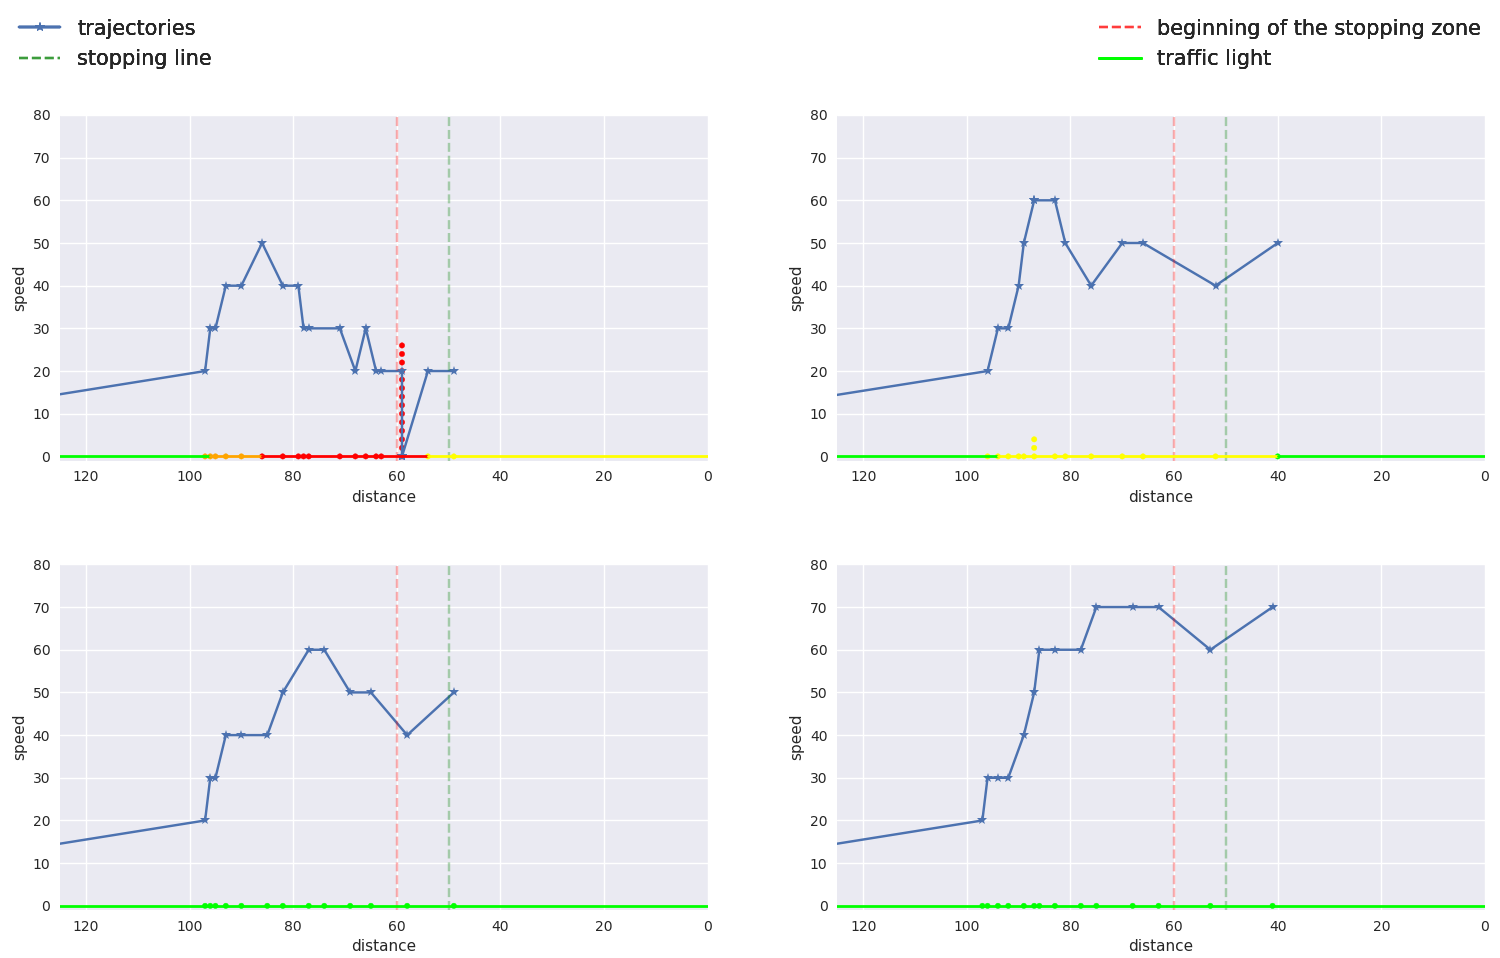
\includegraphics[scale=0.3]{img/new_legend_traj.png}
 \end{frame}
 
\begin{frame}
\frametitle{What could be done next?}
\begin{itemize}
\item we tried to learn with 50 millions iterations ($\geq 60$ hours), but the results were not impressively better than with 10 millions iterations 
\item do grid search in order to find a better reward function
\item generalize the learning to any traffic light
\item Kalman filters to improve measurements 
\item \ldots
\end{itemize}
\end{frame}




\begin{frame}{}
\centering
Thank you for your attention\\ Demo time !\\
\vspace{0.5cm}
\centering
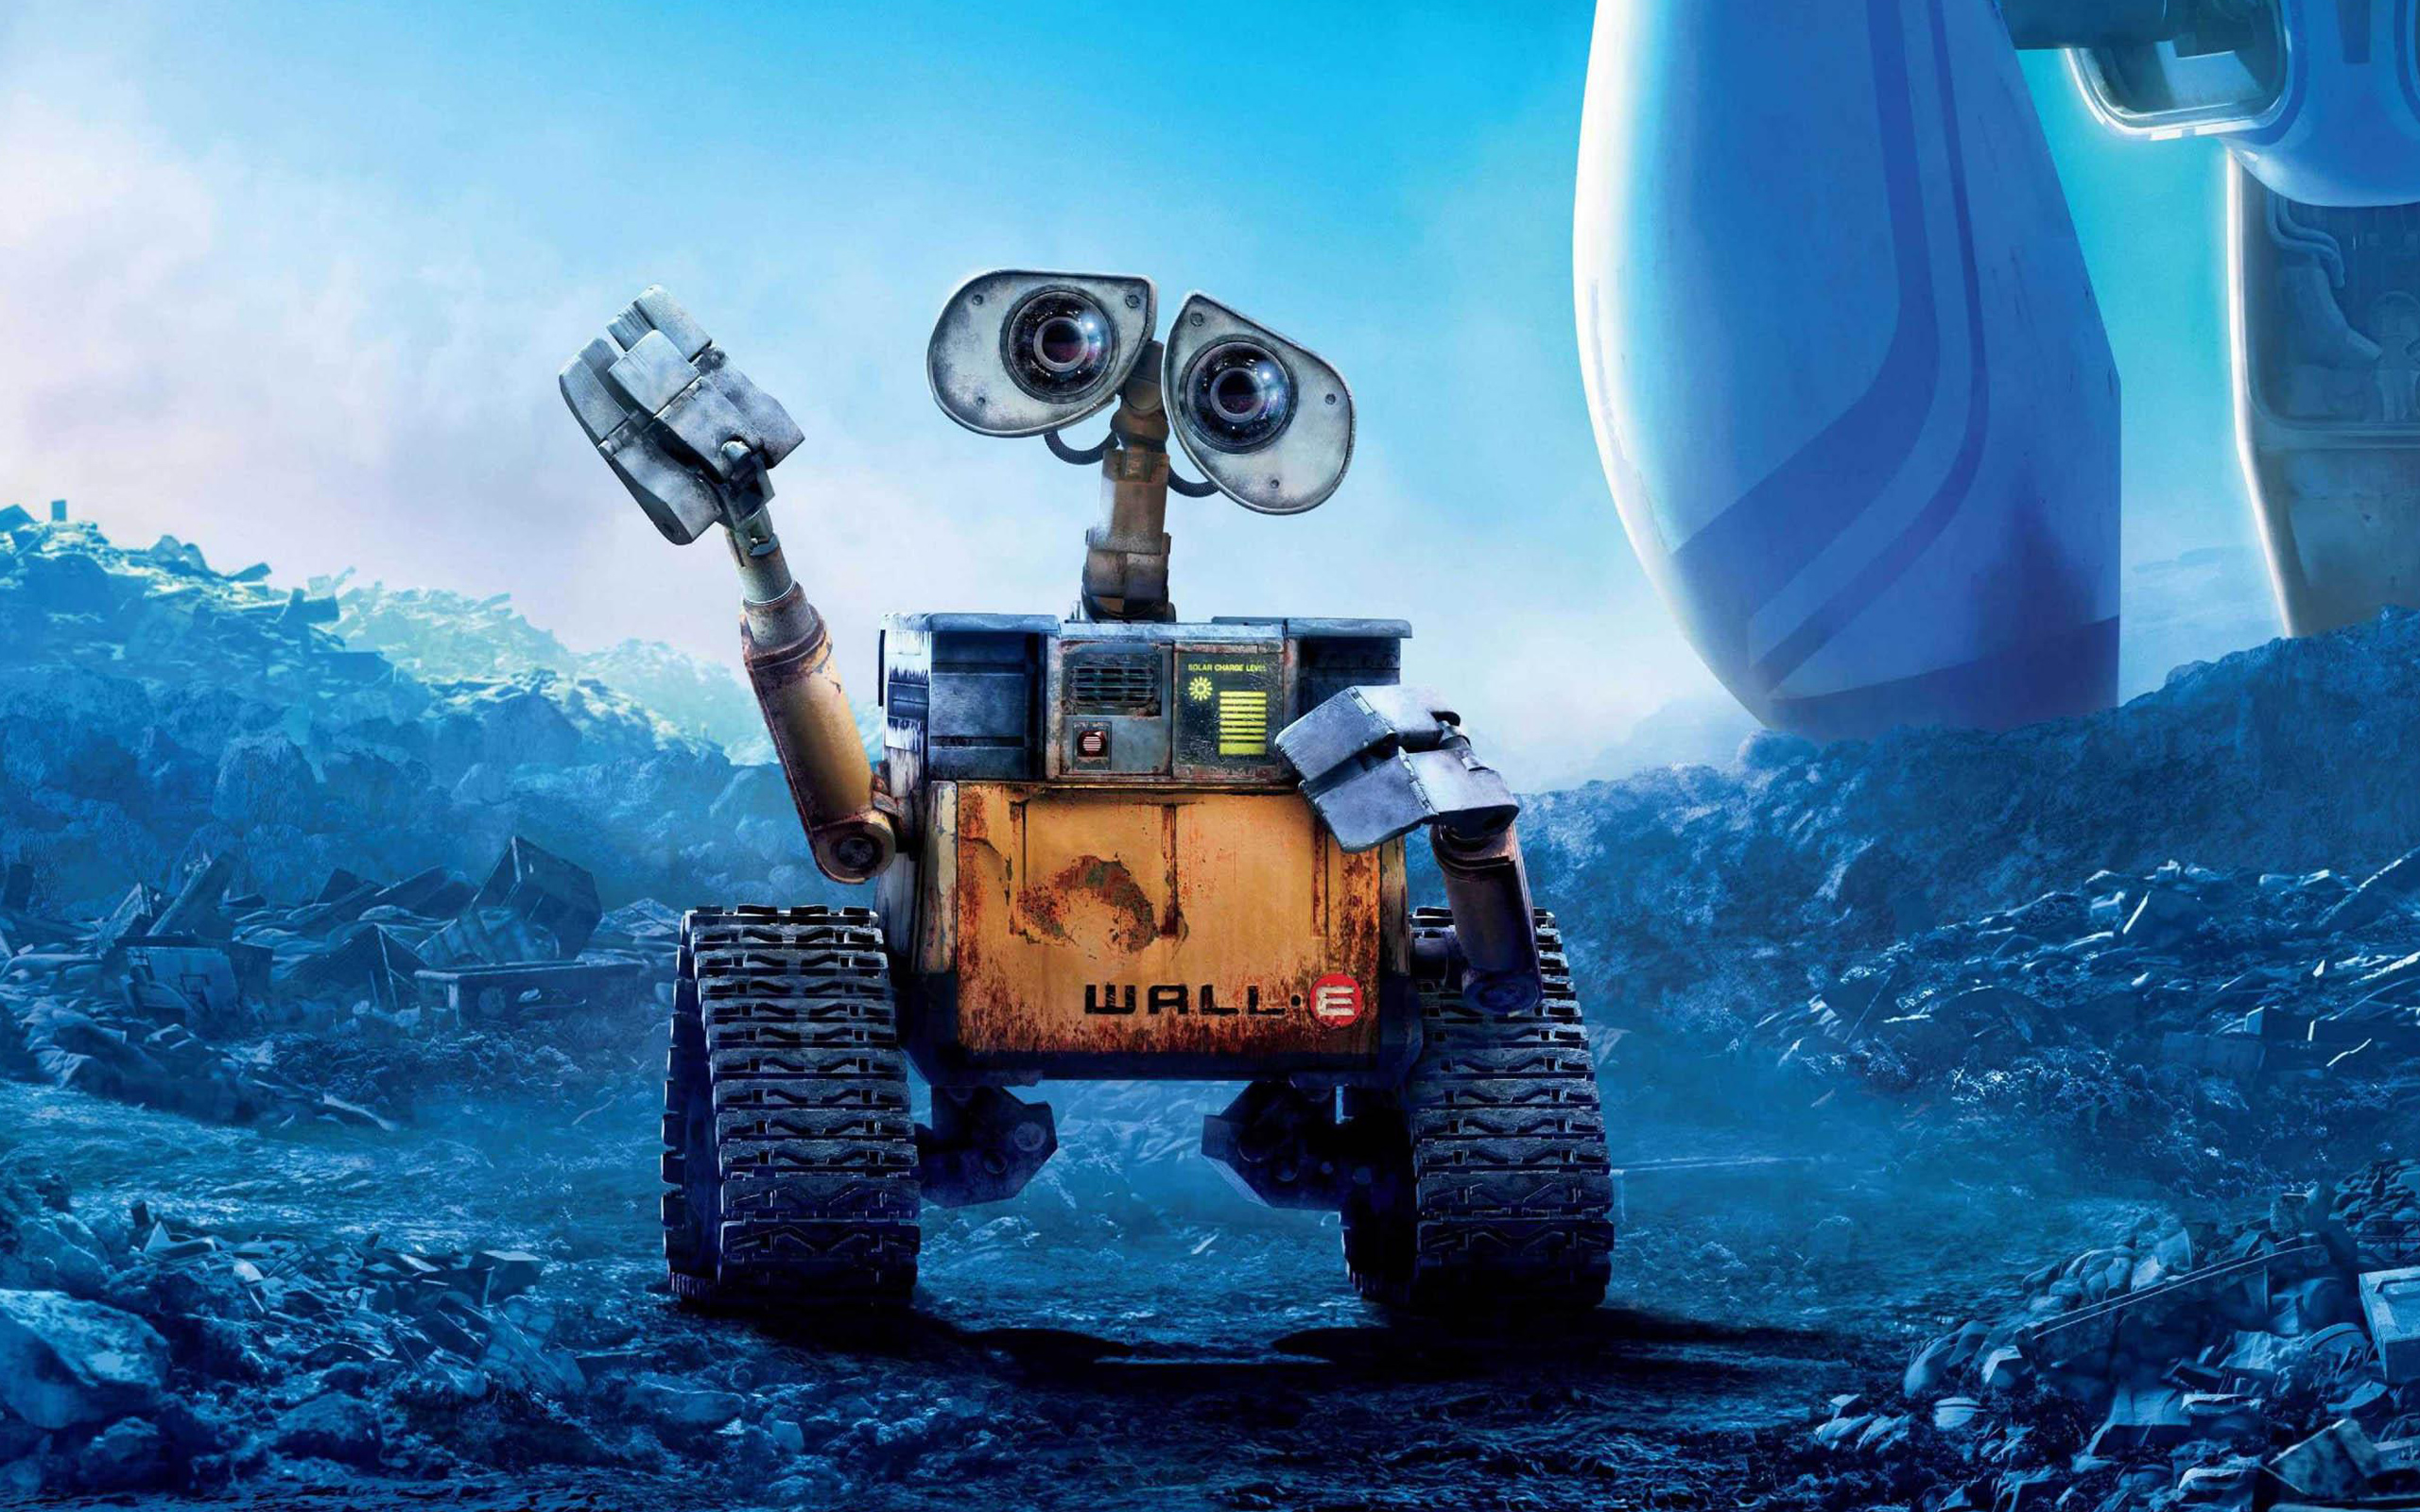
\includegraphics[scale=0.1]{img/walle_end.jpg}
\end{frame}




\end{document}
